\chapter{Software Design}

\section{Use Case}
\begin{figure}[h]
	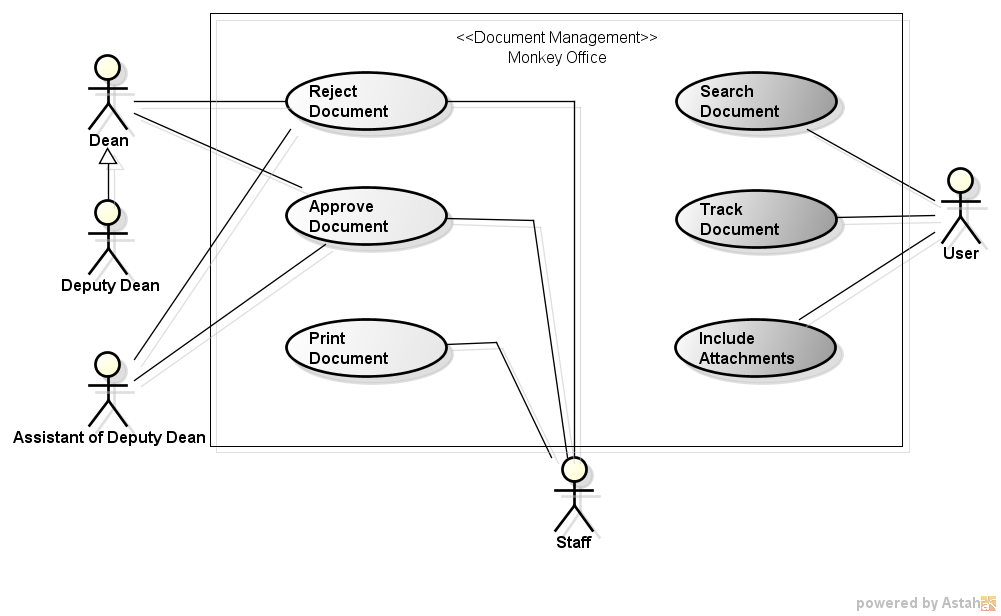
\includegraphics[scale=0.63]{res/Methodology/usecase_diagram}
	\caption{A usecase diagram for Monkey Office}
	\label{fig:usecase-diagram}
\end{figure}
Figure \ref{fig:usecase-diagram} captures system functionalities and requirements represented as \gls{uml} use case diagram.
Table \ref{tbl:actor-description} describes who these type of users are.
\begin{table}
	\centering
	\caption{Type of user and description}
	\label{tbl:actor-description}
	\begin{tabular}{|l|L{7.5cm}|}
		\hline
		Actor & Description \\
		\hline
		Dean & A headmaster of \gls{ic}. \\
		Deputy dean & Dean's assistant who could also be a dean's representative. \\
		Assistant of deputy dean & Deputy dean's assistant who deals with documents that is not critical to \gls{ic}. \\
		Staff & \gls{ic}'s employee in academic department (refer to bottom-most hierarchy in figure \ref{ic-org-sturcture}) \\
		User & A regular user who have an account provided by an administrator to access the system. \\
		\hline
	\end{tabular}
\end{table}

\newcommand{\alreadylogin}{Have already logged in to the system}
\newcommand{\allICPersonel}{
	\begin{itemize}
		\item Dean
		\item Deputy dean
		\item Assistant of deputy dean
		\item Staff
	\end{itemize}
}

\begin{table}
	\caption{Use case: Reject Document}
	
	\begin{tabular}{|l|L{9cm}|}
		\hline
		\textbf{Use Case Name} & Reject Document \\
		\hline
		
		\textbf{Primary Actor} & \allICPersonel \\
		\textbf{Pre-condition} & \alreadylogin. \\
		\textbf{Post-condition} & 
		\begin{itemize}
			\item The system notifies user for a rejected document
			\item The rejected document disappears from the list of pending documents
		\end{itemize} \\
		\textbf{Trigger} & Read the document \\
		\textbf{Basic flow} & 
		\begin{enumerate}
			\item Click a reject button on a designated document.
			\item Click \enquote{Yes} when system asks for a confirmation.
		\end{enumerate} \\
		\hline
	\end{tabular}
\end{table}

\begin{table}
	\caption{Use case: Approve Document}
	\begin{tabular}{|l|L{9cm}|}
		\hline
		\textbf{Use Case Name} & Approve Document \\
		\hline
		
		\textbf{Primary Actor} & \allICPersonel \\
		\textbf{Pre-condition} & \alreadylogin. \\
		\textbf{Post-condition} & 
		\begin{itemize}
			\item The system notifies user for a approve document
			\item The approved document disappears from the list of pending documents
		\end{itemize} \\
		\textbf{Trigger} & Read the document \\
		\textbf{Basic flow} & 
		\begin{enumerate}
			\item Click an approve button on a designated document.
			\item Click \enquote{Yes} when system asks for a confirmation.
		\end{enumerate} \\
		\hline
	\end{tabular}
\end{table}

\begin{table}
	\centering
	\caption{Use case: Print Document}
	\begin{tabular}{|l|L{9cm}|}
		\hline
		\textbf{Use Case Name} & Print Document \\
		\hline
		
		\textbf{Primary Actor} & Staff \\
		\textbf{Pre-condition} & \alreadylogin. \\
		\textbf{Post-condition} & Physical document is print out from the printer successfully. \\
		\textbf{Trigger} & Open the document \\
		\textbf{Basic flow} & 
		\begin{enumerate}
			\item Click \enquote{Print Document} on the main menu.
			\item Select attachments to be print (if any).
			\item Select a printer.
			\item Configure paper size and number of copies as needed.
			\item Click \enquote{Print} to print the document.
		\end{enumerate} \\
		\hline
	\end{tabular}
\end{table}

\section{Storing Digital Documents}
Before storing documents, there are two things to concern.
Firstly, what metadata should be stored alongside the document so that the system can access to the digital file including its attachments.
Attachments are documents.
They can be official or unofficial documents.
Both official and unofficial documents are the same except for one characteristic.
Official documents has a customized identification code as mentioned in table \ref{tbl-doc-subtype}.
Unofficial documents has only regular identification number starting at one and increment by one for each document.
Therefore, the parent document have to store a list of attachments.
That is a list referring to itself.
A class diagram \ref{fig-doc-template} shows 
%\begin{figure*}
%	\label{fig-doc-template}
%	\caption{text}
	%\includegraphics[scale=0.5]{res/Methodology/DocumentTemplating}
%\end{figure*}

Secondly, where digital files should reside in the the server.


\section{Retrieving Digital Documents}

\section{Tracking Digital Documents}